\documentclass{article}
\usepackage{enumitem} % used to minimise list spacing
\usepackage{graphicx} % Required for inserting images
\usepackage{multicol} % Required for multiple columns
\usepackage{caption}   % Required for captions
\usepackage{dirtree}
\usepackage{geometry}
\usepackage{hyperref}
\usepackage{wrapfig}
\geometry{margin=1.25in}

\title{ARM Group Project Report}
\author{Aidan Baker, Yeona Kim, Mruchus Ngo, Hridita Soni}
\date{June 2024}

\begin{document}

\maketitle

\tableofcontents

\section{Assembler}

\subsection{Structure}
The assembler was structured as follows, with .h header files omitted:
\dirtree{%
.1 emulator/.
.2 instructions/.
.3 branchInstr.c.
.3 DataProcessingImm.c.
.3 DataProcessingReg.c.
.3 sdt.c.
.2 fileIO.c.
.2 maps.c.
.2 utilities.c.
.1 assemble.c.
}

Each category of instruction was given its own file as the logic behind converting each instruction to binary was independent of each other. This also made it simple for each member of group to work independently on their assigned instruction type.

Our implementation required a ‘symbol table’ so we decided to use a map to represent this. It was intuitive how the labels would act as the map keys and then memory addresses as values. Therefore, we created a file dedicated to generic map functions which we used to build the symbol table. 

We also separated the code for reading and writing to files as this was unrelated to the code for analysing the assembly.

Additionally, we maintained a file for utility functions applicable to different category of instructions, such as parsing a register to extract the register number from a string). This prevented duplication of code across different instruction files.

\subsection{Implementation}

We decided to perform two passes over the source code. During our first pass we created a symbol table and in the second, we read every line of assembly, analysed whether the code was a label, int directive or an instruction and then applied the appropriate function or to convert the line of assembly into its binary counterpart. We were able to distinguish between different instructions by parsing the operand.

\subsubsection{Instructions}

For each instruction, we first removed the commas and ensured that every non-whitespace character was separated by a space. This guaranteed simple parsing using sscanf. For instructions such as str or ldr, where the address string varied despite having the same opcode, we identified the instruction type by analysing the address format. For example, the presence of a '!' indicated the 'pre-index' addressing mode.

Instructions involving bitwise shifts were easily distinguished by using the return value of sscanf to check the number of operands.

For all instructions, depending on the immediate value, values fetched using labels, and the information extracted from the the parsed registers, the appropriate binary would be generated.\\

\section{Making an LED Flash on a Raspberry Pi}

To make our LED blink we connected the circuit in series and used Pin 7.\\

Our code consisted of the following steps:
\begin{enumerate} [noitemsep]
    \item Clearing out the registers we would be using
    \item Setting Pin 7 to be an output
    \item Setting Pin 7 to a high signal (LED on)
    \item Creating a delay
    \item Setting Pin 7 to a low signal (LED off)
    \item Creating a delay
    \item Repeat steps 2-6 by using a loop
\end{enumerate}

The delay was created by repeatedly incrementing a value stored in a register until it was equal to a sufficiently large number: 0x3ff lsl 12. This consumed processor cycles which created a pause when the LED turned on, and then again when it turned off. \\

\section{Extension - Making a Game Engine for games in the Terminal}

\subsection{Overview}

Initially we decided to make Flappy Bird in the terminal for our extension, however as we progressed it evolved into making a basic generalised game engine using the terminal, by repeatedly printing each frame and having emoji as pixels to create a game 'window'. Examples of this are shown below.

In the end, we made the following games alongside our engine:
\begin{itemize}
    \item Flappy Bird
    \item Pong
    \item 2048
    \item Pacman
    \item Conway's Game of Life (+ colourful version)
\end{itemize}

\begin{multicols}{2}

\subsubsection{Flappy Bird}
This was the initial game we made as it was simple and only had one input, which was a limitation of the initial game engine.\\

\begin{minipage}{\linewidth}
    \centering
    \includegraphics[width=0.8\linewidth]{image.png}
    \captionsetup{type=figure}
    \caption{Flappy Bird}
    \label{fig:game-engine-example}
\end{minipage}

\subsubsection{Pong}
This was another game we developed to learn more about game mechanics and collision detection.\\

\begin{minipage}{\linewidth}
    \centering
    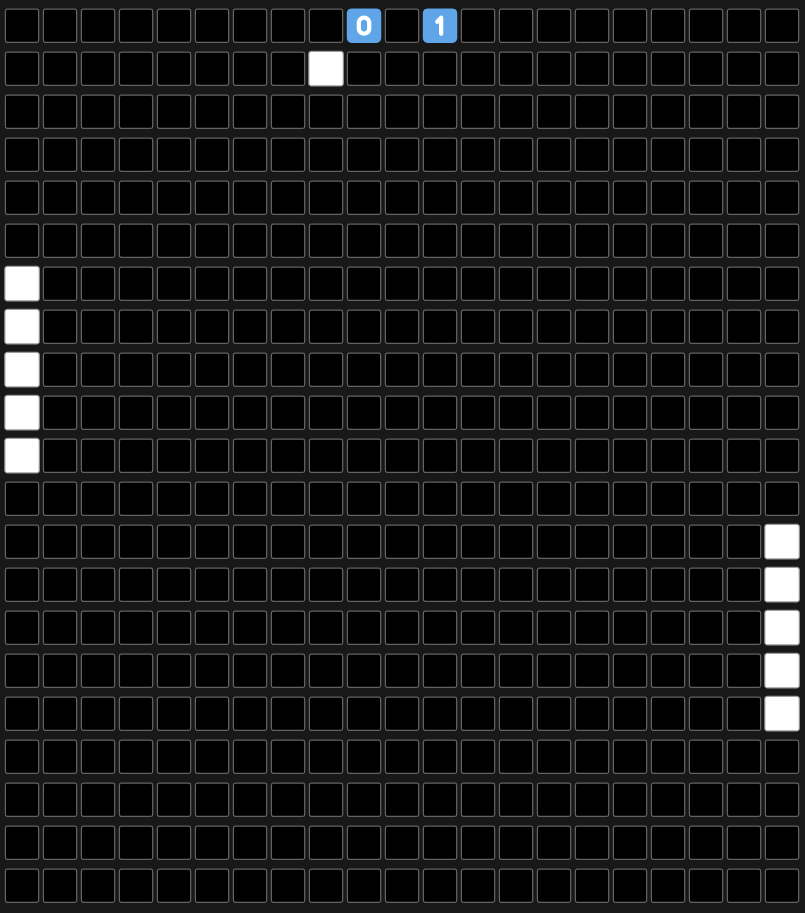
\includegraphics[width=0.8\linewidth]{pong.png}
    \captionsetup{type=figure}
    \caption{Pong}
    \label{fig:enter-label}
\end{minipage}

\end{multicols}

\pagebreak


\begin{multicols}{2}

\subsubsection{2048}
2048 was structured based off structs of blocks which consist of the x, y positions and it's integer value. Depending on the input value, it takes in, all blocks get updated (merging 2 blocks or updating the position of block).  \\

\begin{minipage}{\linewidth}
    \centering
    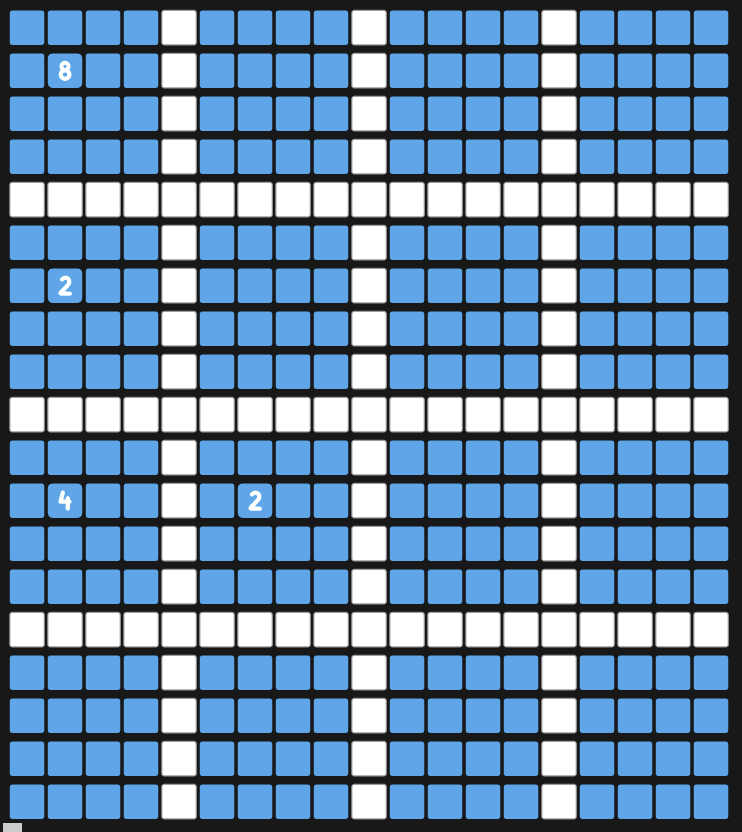
\includegraphics[width=0.8\linewidth]{2048.png}
    \captionsetup{type=figure}
    \caption{2048}
    \label{fig:game-engine-example}
\end{minipage}

\subsubsection{Pacman}
Another game we made using the game engine was Pac-Man. We coded the Pac-Man character as a smiling emoji and the aliens as enemies, which can kill you, and finally stars for the user to pick up points.\\

\begin{minipage}{\linewidth}
    \centering
    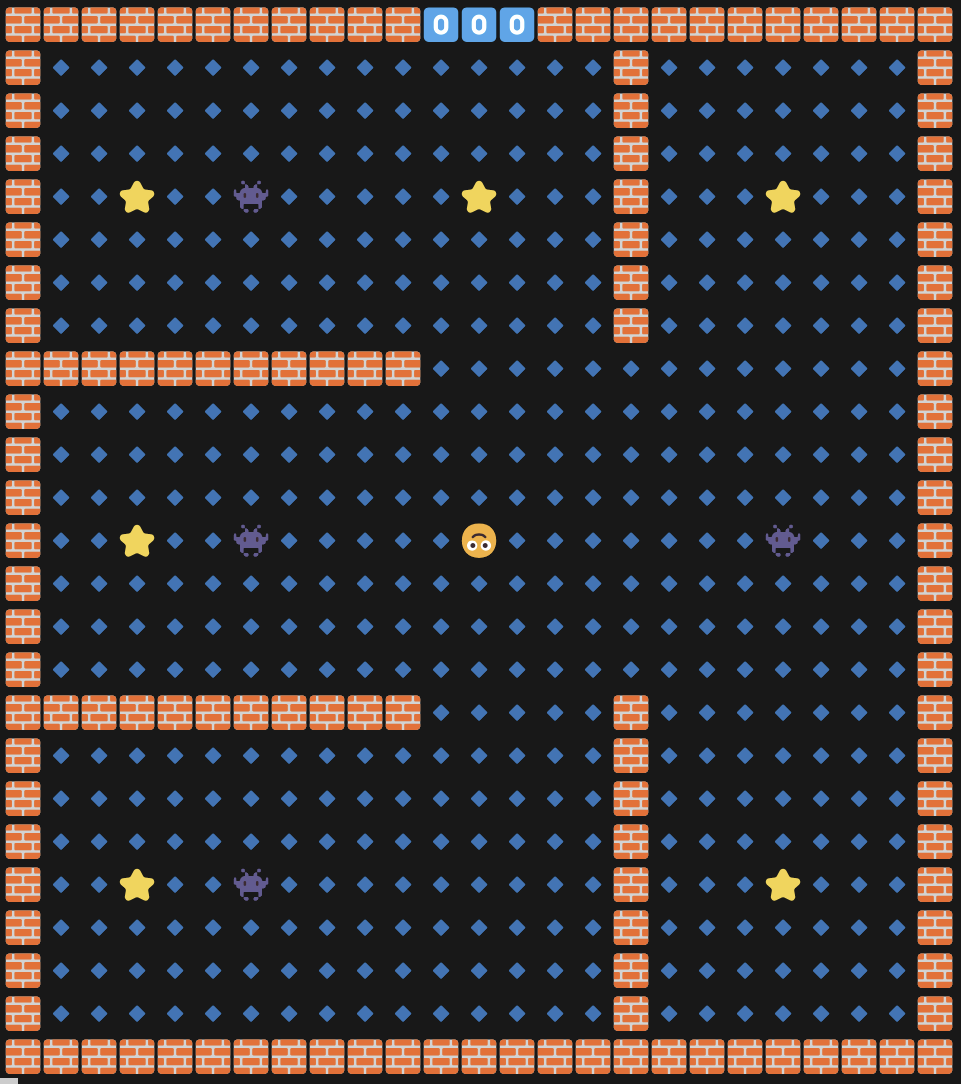
\includegraphics[width=0.8\linewidth]{pacman.png}
    \captionsetup{type=figure}
    \caption{Pacman}
    \label{fig:enter-label}
\end{minipage}

\end{multicols}


\subsubsection{Conway's Game of Life}

\begin{figure}[h]
    \centering
    \begin{minipage}{0.45\textwidth}
        \centering
        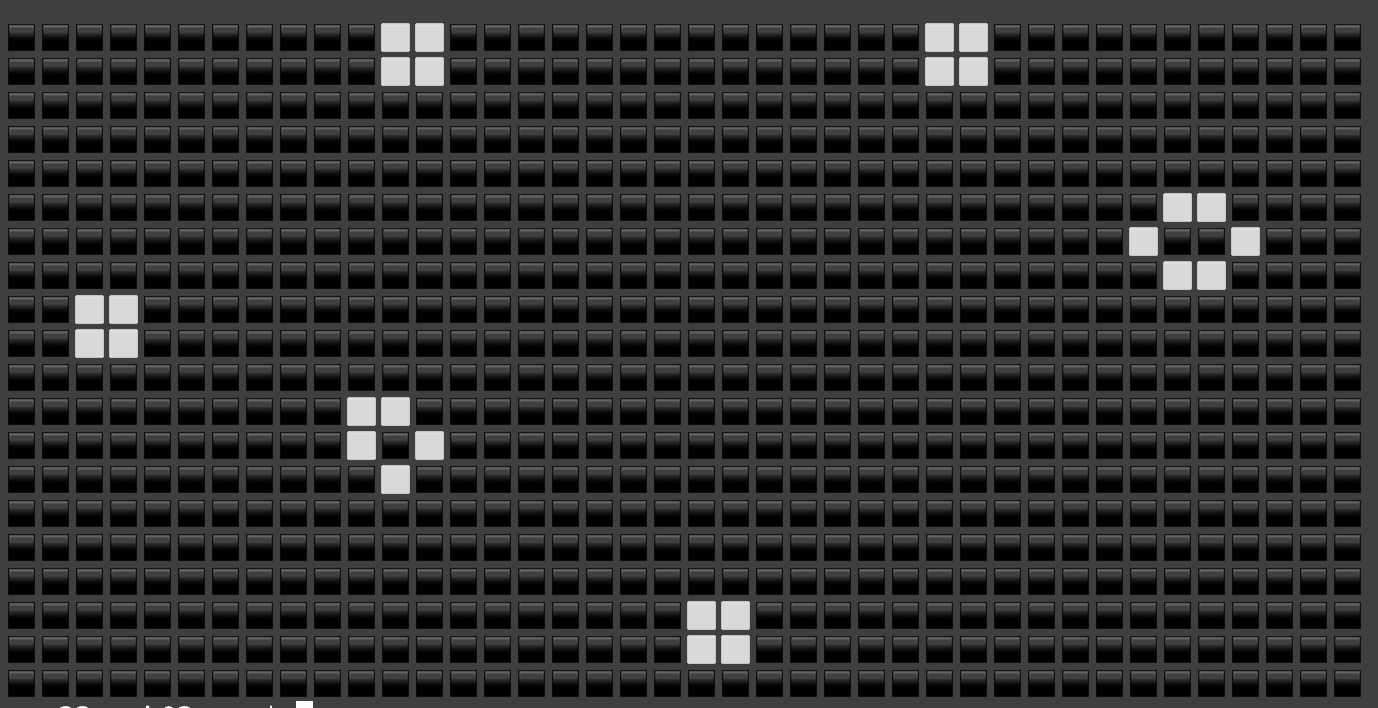
\includegraphics[width=\textwidth]{conway1.png}
        \caption{Conway's Game of Life: Stable configuration in B/W}
        \label{fig:conway1}
    \end{minipage}\hfill
    \begin{minipage}{0.45\textwidth}
        \centering
        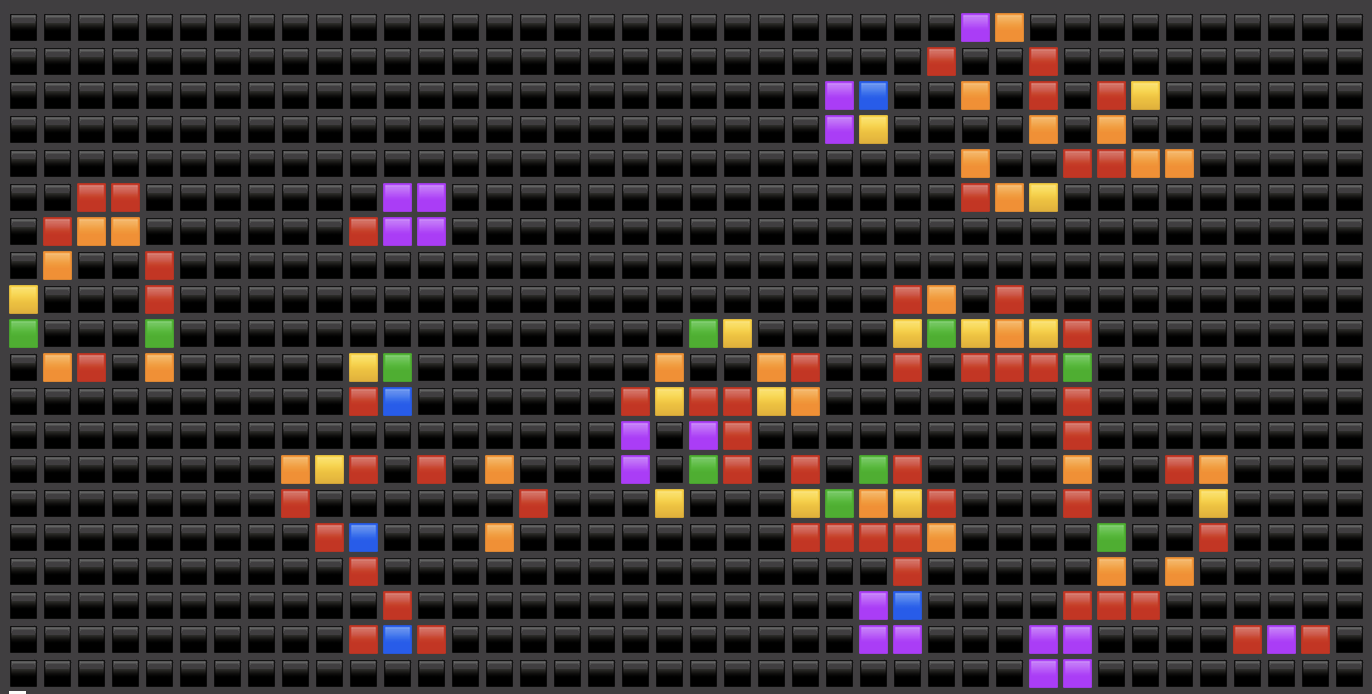
\includegraphics[width=\textwidth]{conway2.png} 
        \caption{Conway's Game of Life: Mid run with colours}
        \label{fig:conway2}
    \end{minipage}
\end{figure}

To increase the variety of our games, we decided to make a simulation game. We chose Conway's Game of Life as the rules were simple but the outcome would complex enough and satisfying to look at.

We decided that it would be inconvenient for start state of the game (determining which cells are dead or alive on the grid) to be decided by the user so we opted to make it randomly generated. Therefore, to allow some level of user interaction we added the following functionalities: q - quit, p - pause/resume, r - reset, c - toggle colours. We also though that it might be interesting to track the stability of the cells and assign a colour based on this. If the cell is red, it has been changing every tick but later colours in the spectrum signify that the cell has been alive for longer.

\subsection{Challenges}
One of the challenges we faced was how to use emoji in C easily seeing as emojis do not fit into the char datatype, which makes manipulating strings containing them much harder. To get around this we made it so every game must provide a 'lookup function' where we actually represent the screen as an array of characters (for example the bird in Flappy Bird maybe represented by a '.'). Then when we print the window to the terminal we use this lookup function to convert a character to a string containing an emoji. This method was still performant and meant that clients of the game engine could easily manipulate pixels on the screen.

Another issue was fetching user input, initially we just used enter as the input, as getc() and other functions will return values when enter is pressed, however this was echoed to the terminal and messed up the printing of the 'screen'. Fortunately we discovered a way to disable the echo to prevent this. Eventually when we generalised the engine for other games we needed more than 1 input button, so we had to make it that user input was returned to the program as it comes instead of all at once when enter was pressed. Luckily there was a way to fix this again by changing the terminal settings.

\subsection{Testing}
To test the game engine we would write very simple programs as we added functionality to the engine. These programs would do basic things using a newly added function, for example setting a pixel on the 'screen'. 

For testing individual games again we played the game and attempted to break it and find cases where the pixels would behave unexpectedly.

\section{Group reflection}
Dividing the work based off instruction categories did not result in even work load, particularly for the assembler, so for the assembler we opted to have a table of specific instructions with each person marking off an instruction as they were working on it. This method meant that we had a roughly equal work load as people who did harder instructions simply did fewer instructions.

After emulator and assembler were completed, Aidan focused on starting the extension by building the game engine, while the rest of the group began writing the assembly code for Part 3. We all worked together to debug, when we came across issues and once we were finished with the assembly code, we each built separate games using the game engine. 

Next time, we aim to be more conscious from the get go that the spec might not divide the work load evenly as we worked more effectively when every member was allowed to pick up unfinished parts after completing their originally assigned section.

In terms of communication, we used a hybrid of sending messages, calling and meeting in person. This worked well for our group as it allowed us to be flexible and still keep everyone up to date with the progress of the project.

\section{Individual reflection}

\subsection{Aidan Baker}
I think I worked well with my group, I felt my views and opinions were sufficiently listened to and debated. Dividing work into sections for each member to implement kept our work quite separated which meant there was little room for disagreement on implementation of specific functions and allowed us to work mostly at our own pace. 
Overall my group was great and I hope I can work with them in the future as we all worked in similar ways.

\subsection{Yeona Kim}
I think I was able to work well and efficiently with our group. I was mostly afriad about having major merging conflicts from using Git. But working on different branches and having our code structure to be very modular made it easier to avoid this issue.\\

Our communication skills definitely shined throughout the project. For example, everyone would be informed whenever something is being merged, or pushed if anyone was working on the same branch. Disscussing new ideas or debugging specific test cases were also simple because everyone was happy to contribute and participate. I found myself to easily share my thoughts with no hesitation and receive constructive feedback leading to faster progresses.

\subsection{Mruchus Ngo}
From the start of the project, I understood that my programming speed was quite slow which made me uncertain as I could not quickly test and integrate my work with the others. However, I compensated for this by putting in the hours and seeking help from other people in the group. The group was willing to review each other's code and assist with debugging which meant that I was never stuck for long. Ultimately, the time I invested in building my code and reading the main utility files paid off, as it gave me a solid understanding of our code's structure and functionality. This came in handy when debugging failing test cases as I was able to identify bugs in code for instructions other than my own.\\

I think I integrated well into the group because we shared similar views on the times at which we would work together and apart and were all willing to maintain a consistent pace. Communication and coordinating sessions to pair program and discuss ideas was also straightforward as everyone would show up to lectures and labs. For any other meetups, groups members were conscientious about checking messages and timings.\\

\subsection{Hridita Soni}
I think this group managed to work impressively together as we communicated well, discussing any complex aspects of the code and ensuring that we covered all parts of the spec’s instructions in the code we produced. We also split the work so that everyone could contribute, allowing me to work in my own time so long as I met the group’s intended targets on time. I found the deadlines we set very useful to ensure I was keeping up to date with my work on the project and to track that our whole group was progressing through each parts of the project well. 

\end{document}
